%======================================================================
% 附录N：等离子体-壁相互作用与偏滤器物理（注明出处）
%======================================================================
% 章标题 \appchapter{附录N：...} 由主文件发出，本文件只提供正文。
% 设计约定：补第 10--11 章之间的空白——磁约束装置的"边界"（SOL / 偏滤器 / 壁侵蚀 / 氚）。
% 版权约定：只借鉴经典教材与文献的物理结论、公式形式与题型，文字与数值由本书自拟并独立复算。
% 数值来源：tools/calc/appN_calc2.py（本附录每一节的关键数字都能由它复现）。

第 10 章讲了芯部怎么点火，第 11 章讲了鞘层与低温等离子体的壁面附近，但两者之间最大的一块空白是：\textbf{芯部产生的功率最终怎么落到壁上、壁能承受多久、燃料会不会被壁吃掉}。这就是磁约束聚变的\textbf{边界物理}（edge physics），也是决定装置能否连续运行的瓶颈——国际热核聚变实验堆（ITER）的设计难点里有相当一部分不在芯部，而在偏滤器靶板与氚滞留上。本附录把这条链条补上。

与相邻附录的分工：附录 J 回答"这个主题该读哪本书的哪一章"；附录 K 是完整解答的\textbf{范例}；附录 L 是\textbf{自测}题库；附录 M 是加热与运行极限的专题深挖；本附录继续专题深挖，但主题换成\textbf{边界与壁}。

\begin{tip}{单位与口径自查}{tip-appn-units}
本附录的数字都可以用计算器复算，仓库脚本 \texttt{appN\_{}calc2.py} 列出了每一步。若结果差一个量级，先查三种口径错位：
\begin{enumerate}[nosep,leftmargin=1.6em]
  \item 功率是"总功率"还是"单靶功率"；
  \item 热流是\textbf{平行}磁力线的 $q_\parallel$ 还是\textbf{垂直}靶面的 $q_\perp$（二者差 $\sin\theta$，$\theta$ 是靶面与磁力线的夹角）；
  \item 时间是"等离子体放电秒数"还是"日历秒数"（每年只有约 $10^{5}\ \mathrm{s}$ 在放电）。
\end{enumerate}
另：公式里的时间单位一律写作 \texttt{yr}（年）与 \texttt{day}（天），避免中文字符落进数学字体造成缺字。
\end{tip}


\section{从芯部到壁：功率账与靶板几何}

边界物理的一切推算都从一张功率账开始。设聚变功率 $P_{\mathrm{fus}}=300\ \mathrm{MW}$，则 $\alpha$ 自加热
\begin{equation}
P_\alpha=\frac15P_{\mathrm{fus}}=60\ \mathrm{MW},
\qquad
P_{\mathrm{heat}}=P_\alpha+P_{\mathrm{ext}}=100\ \mathrm{MW},
\end{equation}
其中外部加热取 $P_{\mathrm{ext}}=40\ \mathrm{MW}$（附录 M 的五种手段之和）。芯部辐射与输运使一部分功率并不流向边界，取辐射份额 $f_{\mathrm{rad}}=30\%$，则真正越过最外闭合磁面（LCFS）进入刮削层的功率是
\begin{equation}
P_{\mathrm{SOL}}=(1-f_{\mathrm{rad}})\,P_{\mathrm{heat}}=70\ \mathrm{MW}.
\label{eq:app-n-psol}
\end{equation}

\textbf{第一步估算：把 $70\ \mathrm{MW}$ 均匀摊到整面壁会怎样？} 取大半径 $R_0=6.2\ \mathrm{m}$、小半径 $a=2\ \mathrm{m}$、拉长比 $\kappa=2$，
\begin{equation}
A_{\mathrm{wall}}\simeq4\pi^2R_0a\kappa\approx979\ \mathrm{m^2},
\qquad
q_{\mathrm{wall}}\simeq\frac{70\ \mathrm{MW}}{979\ \mathrm{m^2}}\approx71.5\ \mathrm{kW/m^2}.
\end{equation}
这个数本身不算大，但它是\textbf{均匀分布}的假设——而磁力线把功率集中到极窄的一条带上，真实壁面承受的不是 $71.5\ \mathrm{kW/m^2}$，而是下面这个数。

\textbf{第二步估算：功率落在多窄的带上？} 刮削层里功率沿磁力线流出，在靶板处沉积的宽度由\textbf{热流宽度} $\lambda_q$ 描述（托卡马克上 $\lambda_q\sim1$--$5\ \mathrm{mm}$，由湍流输运与磁通膨胀共同决定）。设 $\lambda_q=5\ \mathrm{mm}$、磁通膨胀因子 $f_x=5$（偏滤器把磁力线"摊开"的倍数）、内外靶各分一半功率，则单靶湿面积
\begin{equation}
A_{\mathrm{wet}}=2\pi R_0\,\lambda_q f_x
=2\pi(6.2)(5\times10^{-3})(5)\approx0.974\ \mathrm{m^2},
\qquad
q_\parallel=\frac{0.5P_{\mathrm{SOL}}}{A_{\mathrm{wet}}}\approx35.9\ \mathrm{MW/m^2}.
\label{eq:app-n-qpar}
\end{equation}
\textbf{结论一：}同样的 $70\ \mathrm{MW}$，均匀摊开是 $71.5\ \mathrm{kW/m^2}$，沿磁力线集中到靶板是 $35.9\ \mathrm{MW/m^2}$——相差约 $500$ 倍。这就是"边界决定成败"的算术来源。

\textbf{第三步：用几何把 $q_\parallel$ 换成靶面真正承受的 $q_\perp$。} 靶板不与磁力线垂直，而是以很小的掠射角 $\theta$ 相切，则
\begin{equation}
q_\perp=q_\parallel\sin\theta .
\label{eq:app-n-qperp}
\end{equation}
\begin{table}[htbp]
\centering
\small
\caption{倾角对靶面热流的影响（$q_\parallel=35.9\ \mathrm{MW/m^2}$，由式 \eqref{eq:app-n-qpar}）}
\label{tab:app-n-tilt}
\begin{tabular}{@{}lrrrrr@{}}
\toprule
$\theta$（靶面与磁力线夹角） & $90^\circ$ & $10^\circ$ & $5^\circ$ & $3^\circ$ & $1^\circ$ \\
\midrule
$q_\perp\ (\mathrm{MW/m^2})$ & $35.9$ & $6.24$ & $3.13$ & $1.88$ & $0.627$ \\
\bottomrule
\end{tabular}
\end{table}
\textbf{结论二：}把靶板"放平"到与磁力线成 $3^\circ$，热流被压低到 $1.88\ \mathrm{MW/m^2}$——几何杠杆 $1/\sin3^\circ\approx19$ 倍，与磁通膨胀 $f_x=5$ 倍合起来约 $95$ 倍。现代偏滤器正是靠这两级几何杠杆把 $\mathrm{MW/m^2}$ 量级以上的平行热流降到钨靶板可以稳态承受的 $5$--$10\ \mathrm{MW/m^2}$ 以内。

\textbf{出处：}Stangeby《The Plasma Boundary of Magnetic Fusion Devices》第 1--5 章（功率账、$\lambda_q$、磁通膨胀与倾角）；Wesson《Tokamaks》（第 4 版）偏滤器与刮削层一章；Fitzpatrick《Plasma Physics: An Introduction》第 4 章末（鞘层与壁面）。


\section{刮削层与两点模型：靶板温度由上游决定}

上一节用的 $q_\parallel$ 是\textbf{功率账}给出的，但靶板能承受多少热流还取决于\textbf{靶板自己的密度与温度}。鞘层把能量带走的通量由第 11 章的玻姆判据决定：
\begin{equation}
q_\parallel=\gamma\, n_t\, k_BT_t\, c_s(T_t),
\qquad
c_s=\sqrt{\frac{k_BT_t}{m_i}},
\qquad
\gamma\approx7\ (\text{氘等离子体}),
\label{eq:app-n-sheath}
\end{equation}
其中 $\gamma$ 是鞘层热传输系数（离子与电子两个通道之和，含鞘层电势加速的贡献），$n_t$、$T_t$ 是\textbf{靶板处}的密度与温度，$c_s$ 是离子声速（本书约定 $c_s=\sqrt{k_BT_e/m_i}$，与附录 L 第 4 章一致）。

\textbf{关键问题：}$n_t$ 与 $T_t$ 不是自由参数——它们被"上游"（刮削层入口，温度 $T_u$、密度 $n_u$）通过\textbf{平行热传导}与\textbf{压力守恒}锁住。这套关系叫\textbf{两点模型}（two-point model）：能量以电子热传导为主沿磁力线流向靶板，
\begin{equation}
T_u^{7/2}=T_t^{7/2}+\frac{7}{2}\frac{q_\parallel L}{K_{0e}},
\qquad
n_uT_u\simeq n_tT_t \quad(\text{忽略动量损失}),
\label{eq:app-n-twopoint}
\end{equation}
$L$ 是沿磁力线的连接长度，$K_{0e}\simeq2000\ \mathrm{W\,m^{-1}\,eV^{-7/2}}$ 是电子平行热导系数（Spitzer 传导的常用写法，取自 Stangeby）。

把式 \eqref{eq:app-n-twopoint} 与式 \eqref{eq:app-n-sheath} 联立，取 $L=40\ \mathrm{m}$、$q_\parallel=35.9\ \mathrm{MW/m^2}$，对靶板温度求解，得到下表（每一列都是自洽解）：

\begin{table}[htbp]
\centering
\small
\caption{两点模型的自洽解（$q_\parallel=35.9\ \mathrm{MW/m^2}$，$L=40\ \mathrm{m}$，$K_{0e}=2000$）}
\label{tab:app-n-twopoint}
\begin{tabular}{@{}rrrrr@{}}
\toprule
$T_t\ (\mathrm{eV})$ & $c_s\ (\mathrm{m/s})$ & $n_t\ (\mathrm{m^{-3}})$ & $T_u\ (\mathrm{eV})$ & $n_u\ (\mathrm{m^{-3}})$ \\
\midrule
$5$  & $1.55\times10^{4}$ & $4.14\times10^{20}$ & $67.4$ & $3.07\times10^{19}$ \\
$10$ & $2.19\times10^{4}$ & $1.46\times10^{20}$ & $67.4$ & $2.17\times10^{19}$ \\
$15$ & $2.68\times10^{4}$ & $7.97\times10^{19}$ & $67.5$ & $1.77\times10^{19}$ \\
$30$ & $3.79\times10^{4}$ & $2.82\times10^{19}$ & $68.5$ & $1.23\times10^{19}$ \\
$50$ & $4.89\times10^{4}$ & $1.31\times10^{19}$ & $73.5$ & $8.91\times10^{18}$ \\
\bottomrule
\end{tabular}
\end{table}

\textbf{这张表要读出三件事：}
(1) 上游温度几乎不随靶板温度变——$T_u\approx67$--$74\ \mathrm{eV}$。原因是传导项 $\frac72q_\parallel L/K_{0e}\approx2.5\times10^{6}$ 远大于 $T_t^{7/2}\lesssim8\times10^{5}$，也就是\textbf{靶板温度是"被传导关系定出来的小量"}；
(2) 靶板温度越低，需要的靶板密度越高（$T_t=5\ \mathrm{eV}$ 时要 $n_t\approx4\times10^{20}\ \mathrm{m^{-3}}$）——这就是偏滤器的\textbf{高再循环}（high-recycling）工作区间；
(3) 反过来，如果按"低再循环"假设取 $n_t=2\times10^{19}\ \mathrm{m^{-3}}$、$T_t=15\ \mathrm{eV}$，式 \eqref{eq:app-n-sheath} 只给出 $q_\parallel\approx9.0\ \mathrm{MW/m^2}$，比功率账要求的 $35.9\ \mathrm{MW/m^2}$ 低约 $4$ 倍。\textbf{差额只能靠提高靶板密度（高再循环）或靠辐射提前卸掉功率}——这正是下一节"脱靶"的物理动机。

\textbf{顺带得到一个常用的离子通量：}取 $n_t=2\times10^{19}\ \mathrm{m^{-3}}$、$T_t=15\ \mathrm{eV}$，
\begin{equation}
\Gamma_i=n_tc_s\approx5.36\times10^{23}\ \mathrm{m^{-2}\,s^{-1}},
\qquad
E_i\simeq5k_BT_t\approx75\ \mathrm{eV}\ (\text{鞘层加速后的轰击能量}),
\end{equation}
它是下一节算溅射侵蚀的输入。

\textbf{出处：}Stangeby 第 5 章（两点模型、$K_{0e}$ 与高再循环）；Pitcher \& Stangeby, \textit{Plasma Phys.\ Control.\ Fusion} \textbf{39} (1997) 779（刮削层与偏滤器综述）；Wesson 偏滤器章。


\section{脱靶：让杂质把功率"辐射掉"}

上一节末尾留下一笔账：功率账要求 $q_\parallel=35.9\ \mathrm{MW/m^2}$，而倾角只能把它降到 $1.88\ \mathrm{MW/m^2}$；如果靶面允许的上限取 $q_\perp^{\max}=5\ \mathrm{MW/m^2}$（钨单块靶板的稳态量级），则\textbf{还不满足}，差额必须靠\textbf{体辐射}在到达靶板之前卸掉：
\begin{equation}
f_{\mathrm{rad}}=1-\frac{q_\perp^{\max}}{q_\parallel}=1-\frac{5}{35.9}\approx0.861
\qquad\Longrightarrow\qquad
P_{\mathrm{rad}}^{\mathrm{div}}=f_{\mathrm{rad}}\times35\ \mathrm{MW}\approx30.1\ \mathrm{MW}.
\label{eq:app-n-frad}
\end{equation}
也就是说，偏滤器必须把\textbf{单靶 $86\%$ 的入射功率变成光子}，只让剩下 $14\%$ 打到靶板上——这就是\textbf{脱靶}（detachment）运行点的定义：靶板前的等离子体温度降到几 $\mathrm{eV}$，杂质（氮、氖、氩）在这个低温区辐射极强，把能量以线辐射与轫致辐射的形式散布到整面壁上。

\textbf{需要多少杂质？} 体辐射功率为
\begin{equation}
P_{\mathrm{rad}}=n_en_{\mathrm{imp}}L_z(T_e)\,V,
\label{eq:app-n-lz}
\end{equation}
其中 $L_z$ 是杂质冷却速率系数（$\mathrm{W\,m^3}$，强烈依赖温度，在 $5$--$10\ \mathrm{eV}$ 附近有峰值）。取 $n_e=10^{20}\ \mathrm{m^{-3}}$、偏滤器体积 $V=20\ \mathrm{m^3}$，反解所需杂质密度：
\begin{table}[htbp]
\centering
\small
\caption{脱靶所需杂质比例对 $L_z$ 的敏感性（$P_{\mathrm{rad}}=30.1\ \mathrm{MW}$，$n_e=10^{20}\ \mathrm{m^{-3}}$，$V=20\ \mathrm{m^3}$）}
\label{tab:app-n-impurity}
\begin{tabular}{@{}lrr@{}}
\toprule
低温辐射系数 $L_z\ (\mathrm{W\,m^3})$ & 所需 $n_{\mathrm{imp}}\ (\mathrm{m^{-3}})$ & 杂质比例 $n_{\mathrm{imp}}/n_e$ \\
\midrule
$3\times10^{-32}$（强辐射区） & $5.02\times10^{17}$ & $0.50\%$ \\
$3\times10^{-33}$（弱辐射区） & $5.02\times10^{18}$ & $5.0\%$ \\
\bottomrule
\end{tabular}
\end{table}
\textbf{教学要点：}同样的辐射功率，$L_z$ 差一个量级，所需杂质比例就差一个量级（$0.5\%$ 对 $5\%$）。而杂质比例不能任意提高——杂质会稀释燃料、并在芯部造成辐射损失（第 10 章的 $P_{\mathrm{loss}}$）。所以脱靶运行是\textbf{在"辐射足够"与"别把芯部也冷却"之间走钢丝}，这也是为什么现代偏滤器研究大量依赖 $L_z$ 的精确数据。

\begin{warning}{把"脱靶"当成"关掉热流"}{warn:appn-detach}
脱靶并不是让功率消失，而是把它\textbf{提前变成辐射}：辐射是各向同性的，落到整面壁上（面积约 $979\ \mathrm{m^2}$）而不是 $1\ \mathrm{m^2}$ 的靶带上，所以壁面能承受。代价是：(1) 靶板前温度过低时，等离子体"脱离"靶板，打击点位置与粒子排出通道都会改变；(2) 辐射区若上移到 X 点以上（"MARFE"），会直接冷却芯部边缘并可能触发密度极限。脱靶是一个\textbf{运行窗口}，不是开关。
\end{warning}

\textbf{出处：}Stangeby 第 4--6 章（脱靶与杂质辐射）；Pitcher \& Stangeby (1997) 综述中的辐射功率账；Wesson 偏滤器章。


\begin{figure}[htbp]
\centering
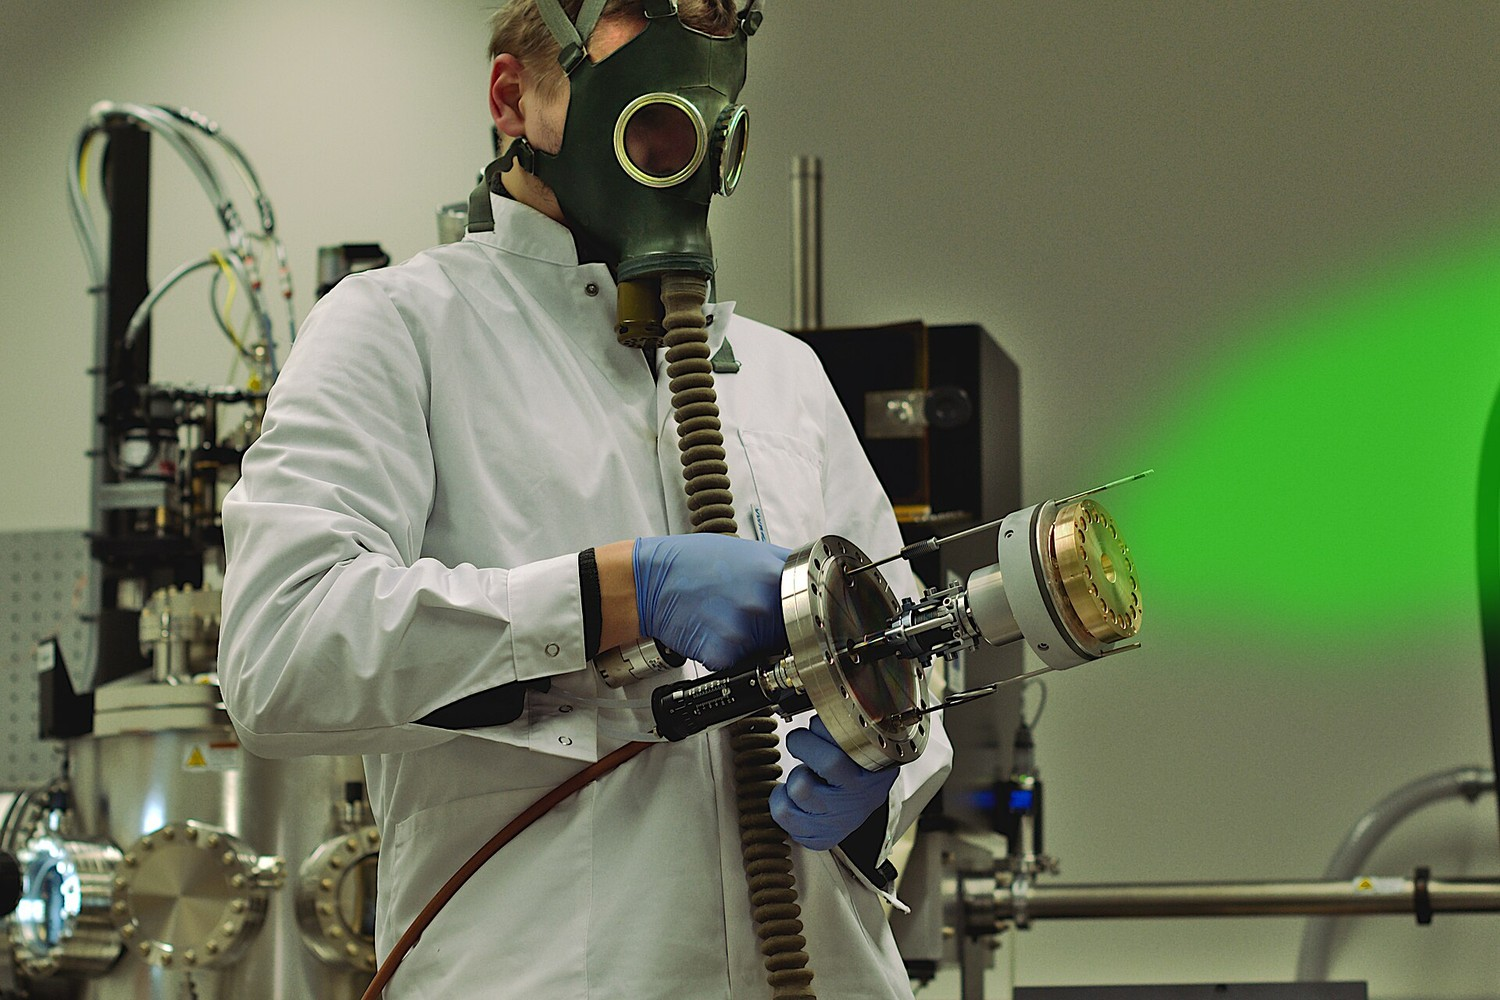
\includegraphics[width=0.78\textwidth]{../figures/sputter_gun.jpg}
\caption{把溅射拿来做工艺：磁控溅射枪。同一套物理在这里被反过来用：等离子体里的离子被鞘层加速后打到靶上，把靶原子撞出来沉积到别处——壁上的溅射侵蚀与这里的镀膜是同一件事的两种结果。}
\label{fig:photo-appn2}
\figsource{Tavoromann，CC BY-SA 4.0（Wikimedia Commons），链接见 figures/CREDITS.md。}
\end{figure}

\section{溅射与侵蚀：稳态不致命，ELM 才致命}

靶板材料（现代装置用钨）被离子轰击会逐层剥落，机制是\textbf{物理溅射}：入射离子把动量传给表面原子，使其获得超过表面结合能的能量而离开表面。单位入射离子打出的靶原子数叫\textbf{溅射产额} $Y$，则侵蚀速率
\begin{equation}
\dot{d}=\frac{Y\,\Gamma_i}{n_{\mathrm{W}}},
\qquad
n_{\mathrm{W}}\approx6.3\times10^{28}\ \mathrm{m^{-3}}\ (\text{钨的原子密度}).
\label{eq:app-n-erosion}
\end{equation}

\textbf{(1) 稳态轰击（$E_i\approx75\ \mathrm{eV}$）：} 取氘离子对钨的产额 $Y\approx10^{-5}$（$75\ \mathrm{eV}$ 远低于钨的溅射阈值 $\sim200\ \mathrm{eV}$，产额很小），代入 $\Gamma_i=5.36\times10^{23}\ \mathrm{m^{-2}\,s^{-1}}$：
\begin{equation}
\dot{d}=\frac{10^{-5}\times5.36\times10^{23}}{6.3\times10^{28}}
\approx8.5\times10^{-11}\ \mathrm{m/s}=0.085\ \mathrm{nm/s}.
\end{equation}
按"每年 $10^{4}$ 次放电、每次 $10\ \mathrm{s}$"（即每年约 $10^{5}\ \mathrm{s}$ 等离子体时间，而不是 $3.15\times10^{7}\ \mathrm{s}$ 日历秒）折算：
\begin{equation}
\dot{d}_{\mathrm{steady}}\approx8.5\ \mathrm{\mu m/yr}\ (\text{无再沉积}),
\qquad
\approx0.85\ \mathrm{\mu m/yr}\ (\text{再沉积 $90\%$}),
\end{equation}
$5\ \mathrm{mm}$ 厚的钨靶板在这种速率下寿命约 $5900$ 年——\textbf{稳态溅射对钨靶板几乎无威胁}。

\textbf{(2) 边缘局域模（ELM）轰击（$E_i\sim300\ \mathrm{eV}$）：} 情况完全反过来。单次 ELM 把 $1\ \mathrm{MJ/m^2}$ 的能量在 $0.3\ \mathrm{ms}$ 内砸到靶板上，离子通量为
\begin{equation}
\Gamma_{\mathrm{ELM}}=\frac{10^{6}\ \mathrm{J/m^2}}{300\ \mathrm{eV}}\approx2.08\times10^{22}\ \mathrm{m^{-2}},
\qquad
Y_{\mathrm{ELM}}\approx10^{-3},
\end{equation}
单次 ELM 的侵蚀深度 $d_{\mathrm{ELM}}\approx0.33\ \mathrm{nm}$；每次放电 $1000$ 次 ELM $\Rightarrow0.33\ \mathrm{\mu m}$；每年 $10^{4}$ 次放电 $\Rightarrow$
\begin{equation}
\dot{d}_{\mathrm{ELM}}\approx3.30\ \mathrm{mm/yr}\ (\text{无再沉积}),
\qquad
\approx0.330\ \mathrm{mm/yr}\ (\text{再沉积 $90\%$}),
\end{equation}
$5\ \mathrm{mm}$ 靶板寿命只剩约 $15$ 年——\textbf{ELM 造成的侵蚀比稳态高约 $390$ 倍}。

\textbf{结论：}决定钨靶板寿命的不是"稳态热流与稳态溅射"，而是\textbf{瞬态事件}。因此现代装置的壁寿命设计必须包含 ELM 缓解（弹丸注入提高 ELM 频率、共振磁扰动 RMP 抑制 ELM，或完全无 ELM 的运行模式），这条结论与下一节的热负荷结论完全同源。

\textbf{出处：}Stangeby 第 3、6 章（溅射产额与再沉积）；Roth 等，\textit{J.\ Nucl.\ Mater.} 系列溅射产额数据汇编（氘/杂质对钨、铍、碳）；Federici 等关于等离子体-壁相互作用与靶板寿命的综述；Wesson 偏滤器章。


\section{边缘局域模（ELM）与瞬态热负荷}

\textbf{什么是 ELM。} 高约束模式（H 模）边缘存在一个输运垒（"台基"，pedestal），它把边缘压强梯度抬到\textbf{剥离-气球模}（peeling-ballooning）稳定性边界；一旦越界，边缘就会周期性地失稳，把台基储存能量的一小部分在亚毫秒内抛到偏滤器上，这就是 I 型 ELM。

\textbf{第一步：台基里存了多少能量？} 用零维能量内容
\begin{equation}
W_{\mathrm{th}}=3n k_BT V,
\end{equation}
取 $n=10^{20}\ \mathrm{m^{-3}}$、$T=10\ \mathrm{keV}$、$V=840\ \mathrm{m^3}$：
\begin{equation}
W_{\mathrm{th}}=3(10^{20})(10^{4}\times1.602\times10^{-19})(840)\approx4.04\times10^{8}\ \mathrm{J}=404\ \mathrm{MJ}.
\end{equation}
（与 ITER 量级 $350\ \mathrm{MJ}$ 相符，可作数量级校验。）

\textbf{第二步：单次 ELM 抛掉多少、砸到哪里？} 取 $\Delta W_{\mathrm{ELM}}/W_{\mathrm{th}}=10\%$，即 $40.4\ \mathrm{MJ}$；其中 $50\%$ 在途中被辐射掉，剩余 $20.2\ \mathrm{MJ}$ 分布在 $20\ \mathrm{m^2}$ 的湿面积上，历时 $0.3\ \mathrm{ms}$：
\begin{equation}
q_{\mathrm{ELM}}\simeq\frac{20.2\ \mathrm{MJ}}{20\ \mathrm{m^2}\times0.3\ \mathrm{ms}}
\approx3.4\times10^{9}\ \mathrm{W/m^2}=3.4\ \mathrm{GW/m^2}.
\label{eq:app-n-qelm}
\end{equation}
与稳态 $q_\perp=1.88\ \mathrm{MW/m^2}$（表 \ref{tab:app-n-tilt}）相比：
\begin{equation}
\frac{q_{\mathrm{ELM}}}{q_\perp}\approx1.8\times10^{3}.
\end{equation}

\textbf{第三步：这个数字对材料意味着什么？} $3.4\ \mathrm{GW/m^2}$ 已超过钨的熔融阈值量级（熔点 $3695\ \mathrm{K}$，瞬态熔融阈值与脉冲长度有关，约 $\mathrm{GW/m^2}$ 量级），所以 ELM 是\textbf{瞬态损伤}（熔融、开裂、溅射暴增）的主因。这就解释了为什么上面的侵蚀账里 ELM 比稳态高两个多量级，也解释了 ELM 缓解为何是 ITER 的关键工程课题：把单次 $\Delta W_{\mathrm{ELM}}$ 压到 $W_{\mathrm{th}}$ 的 $0.5\%$ 以下，或把 ELM 频率提高到每次抛出的能量足够小。

\textbf{与附录 M 的呼应：}附录 M 讲的是"怎么把功率加进芯部"，本附录讲的是"这些功率最终砸在哪里"。同一个 $70\ \mathrm{MW}$（式 \eqref{eq:app-n-psol}），芯部要的是"进得去"，边界要的是"出得来且别砸坏壁"——两者构成聚变装置的两端约束。

\textbf{出处：}Loarte 等，\textit{Phys.\ Scr.}（2007）关于 ELM 与瞬态热负荷的综述；Wesson 第 14 章（H 模与 ELM）；Leonard 关于偏滤器与现代边界运行的综述；ITER 设计基准文档（Physics Basis）中的瞬态热负荷限值。


\section{燃料滞留、氚自持与增殖比}

\textbf{(1) 氚消耗率。} 每次 D--T 聚变释放 $17.6\ \mathrm{MeV}$，同时消耗一个氚核：
\begin{equation}
\dot{N}_{\mathrm{T}}=\frac{P_{\mathrm{fus}}}{17.6\ \mathrm{MeV}}
=\frac{P_{\mathrm{fus}}}{2.82\times10^{-12}\ \mathrm{J}}.
\end{equation}
$P_{\mathrm{fus}}=500\ \mathrm{MW}$ 时 $\dot{N}_{\mathrm{T}}\approx1.77\times10^{20}\ \mathrm{s^{-1}}$，折合
\begin{equation}
\dot{m}_{\mathrm{T}}\approx76.7\ \mathrm{g/day}\ (\text{连续满功率运行}),
\qquad
46.0\ \mathrm{g/day}\ (P_{\mathrm{fus}}=300\ \mathrm{MW}).
\label{eq:app-n-tburn}
\end{equation}
\textbf{(2) 滞留为什么是硬约束。} 氚会滞留在壁与共沉积层里（共沉积、注入、缺陷捕获）。若滞留比例为 $1\%$：
\begin{equation}
\dot{m}_{\mathrm{ret}}=0.767\ \mathrm{g/day}\ (500\ \mathrm{MW}),
\qquad
\frac{1\ \mathrm{kg}}{0.767\ \mathrm{g/day}}\approx3.6\ \mathrm{yr}
\end{equation}
就会触到"装置内氚库存 $1\ \mathrm{kg}$"的安全限值——而装置的设计寿命是十年以上。反过来算：要在十年内把累计滞留压在 $1\ \mathrm{kg}$ 以内，滞留比例必须低于
\begin{equation}
\frac{1000\ \mathrm{g}/(10\times365\ \mathrm{day})}{76.7\ \mathrm{g/day}}\approx0.36\%.
\label{eq:app-n-retlimit}
\end{equation}
$P_{\mathrm{fus}}=300\ \mathrm{MW}$ 时放宽到约 $0.60\%$（对应约 $6.0$ 年触顶）。这就是"燃料滞留"从工程细节变成\textbf{设计约束}的原因。

\textbf{(3) 别忘了衰变。} 氚半衰期 $12.32$ 年，衰变常数 $\lambda=\ln2/12.32\ \mathrm{yr}\approx1.54\times10^{-4}\ \mathrm{day^{-1}}$。$1\ \mathrm{kg}$ 库存每天自发衰变
\begin{equation}
\dot{m}_{\mathrm{decay}}=1000\ \mathrm{g}\times1.54\times10^{-4}\ \mathrm{day^{-1}}\approx0.154\ \mathrm{g/day},
\end{equation}
与式 \eqref{eq:app-n-retlimit} 允许的 $0.27\ \mathrm{g/day}$ 同量级——也就是说\textbf{库存本身的衰变就是必须计入的损失通道}。

\textbf{(4) 增殖比 TBR。} 氚必须"边烧边造"：包层里的 $^{6}\mathrm{Li}(n,\alpha)\mathrm{T}$ 与 $^{7}\mathrm{Li}(n,n'\alpha)\mathrm{T}$ 反应把中子变成氚。由于中子会被结构材料吸收、从缝隙漏掉，且一个中子最多产生一个氚，工程上要求
\begin{equation}
\mathrm{TBR}=\frac{\text{产生的氚}}{\text{消耗的氚}}\gtrsim1.05\text{--}1.15,
\end{equation}
余量用于补偿吸收与泄漏损失，并需要铍或铅作为\textbf{中子倍增剂}。$\mathrm{TBR}<1$ 的装置无论芯部多好都不可能自持——这是与"点火条件"完全独立、同等硬的一条约束。

\textbf{与全书其他部分的连线：}氚消耗率由第 10 章的 $P_{\mathrm{fus}}$ 决定；滞留与壁材料由本附录 \S N.4 的溅射/再沉积决定；而 TBR 属于包层与中子学，本书不展开，但给出量级与判据。

\textbf{出处：}Wesson 第 1 章与第 14 章（氚消耗与增殖）；ITER 设计基准文档（库存限值与 TBR 要求）；Stangeby 第 1 章（共沉积与燃料滞留的机制综述）。


\section{六道估算练习（含答案）}

以下六题全部只用到本附录的公式与量级，建议\textbf{先自己算到量级，再对答案}；答案里的每一步都能在仓库脚本 \texttt{appN\_{}calc2.py} 中复现。

\begin{enumerate}
\item \textbf{（边界功率账）} 某装置 $P_{\mathrm{fus}}=300\ \mathrm{MW}$、$P_{\mathrm{ext}}=40\ \mathrm{MW}$、芯部辐射 $30\%$。求 $P_{\mathrm{SOL}}$；再取 $\lambda_q=5\ \mathrm{mm}$、$f_x=5$、内外靶各半，求 $q_\parallel$ 与 $\theta=3^\circ$ 时的 $q_\perp$。\\
\textbf{答案：}$P_\alpha=60\ \mathrm{MW}$，$P_{\mathrm{heat}}=100\ \mathrm{MW}$，$P_{\mathrm{SOL}}=70\ \mathrm{MW}$；$A_{\mathrm{wet}}=2\pi(6.2)(5\times10^{-3})(5)=0.974\ \mathrm{m^2}$，$q_\parallel=35\ \mathrm{MW}/0.974\ \mathrm{m^2}\approx35.9\ \mathrm{MW/m^2}$；$q_\perp=35.9\times\sin3^\circ\approx1.88\ \mathrm{MW/m^2}$。

\item \textbf{（鞘层热传输）} 靶板 $n_t=2\times10^{19}\ \mathrm{m^{-3}}$、$T_t=15\ \mathrm{eV}$、$\gamma=7$，氘等离子体。求 $c_s$ 与 $q_\parallel$，并与第 1 题的 $35.9\ \mathrm{MW/m^2}$ 比较，说明差额意味着什么。\\
\textbf{答案：}$c_s=\sqrt{k_BT_t/m_D}=\sqrt{15\times1.602\times10^{-19}/3.344\times10^{-27}}\approx2.68\times10^{4}\ \mathrm{m/s}$；$q_\parallel=\gamma n_tk_BT_tc_s=7(2\times10^{19})(15\times1.602\times10^{-19})(2.68\times10^{4})\approx9.0\ \mathrm{MW/m^2}$，仅为功率账要求的 $1/4$。差额说明靶板必须进入\textbf{高再循环}（密度升到 $10^{20}$ 量级、温度降到几 $\mathrm{eV}$），或由辐射提前卸掉功率（\S N.3）。

\item \textbf{（两点模型）} 由上题条件（$q_\parallel=35.9\ \mathrm{MW/m^2}$、$L=40\ \mathrm{m}$、$K_{0e}=2000\ \mathrm{W\,m^{-1}\,eV^{-7/2}}$、$T_t=15\ \mathrm{eV}$）求上游温度 $T_u$，再由压力守恒求 $n_u$。\\
\textbf{答案：}$T_t^{7/2}=15^{3.5}\approx1.31\times10^{4}$，$\frac72q_\parallel L/K_{0e}=3.5(3.59\times10^{7})(40)/2000\approx2.51\times10^{6}$，故 $T_u^{7/2}\approx2.53\times10^{6}$，$T_u\approx67.5\ \mathrm{eV}$；$n_u=n_tT_t/T_u\approx7.97\times10^{19}\times15/67.5\approx1.77\times10^{19}\ \mathrm{m^{-3}}$。注意 $T_u$ 对 $T_t$ 极不敏感（表中 $5$--$50\ \mathrm{eV}$ 都给出 $T_u\approx67$--$74\ \mathrm{eV}$）。

\item \textbf{（脱靶与杂质）} 单靶入射 $35\ \mathrm{MW}$，靶面允许 $5\ \mathrm{MW/m^2}$。求需要辐射掉的比例与功率；再取 $n_e=10^{20}\ \mathrm{m^{-3}}$、$V=20\ \mathrm{m^3}$、$L_z=3\times10^{-32}\ \mathrm{W\,m^3}$，求所需杂质比例；若 $L_z$ 低一个量级，结果如何？\\
\textbf{答案：}入射等效热流 $35\ \mathrm{MW}/0.974\ \mathrm{m^2}=35.9\ \mathrm{MW/m^2}$，$f_{\mathrm{rad}}=1-5/35.9\approx86\%$，即 $P_{\mathrm{rad}}\approx30\ \mathrm{MW}$；由 $n_{\mathrm{imp}}=P_{\mathrm{rad}}/(n_eL_zV)=30\times10^{6}/(10^{20}\times3\times10^{-32}\times20)\approx5.0\times10^{17}\ \mathrm{m^{-3}}$，比例 $0.50\%$；$L_z$ 降十倍则需 $5.0\%$——杂质比例与 $L_z$ 成反比，这就是 $L_z$ 数据重要的原因。

\item \textbf{（ELM 瞬态热负荷）} $n=10^{20}\ \mathrm{m^{-3}}$、$T=10\ \mathrm{keV}$、$V=840\ \mathrm{m^3}$，求 $W_{\mathrm{th}}$；取 $\Delta W_{\mathrm{ELM}}/W_{\mathrm{th}}=10\%$、途中辐射 $50\%$、湿面积 $20\ \mathrm{m^2}$、历时 $0.3\ \mathrm{ms}$，求峰值热流，并与稳态 $1.88\ \mathrm{MW/m^2}$ 比较。\\
\textbf{答案：}$W_{\mathrm{th}}=3nk_BTV=3(10^{20})(1.602\times10^{-15})(840)\approx4.04\times10^{8}\ \mathrm{J}=404\ \mathrm{MJ}$；$\Delta W_{\mathrm{ELM}}=40.4\ \mathrm{MJ}$，$q_{\mathrm{ELM}}=0.5(40.4\times10^{6})/(20\times3\times10^{-4})\approx3.4\times10^{9}\ \mathrm{W/m^2}=3.4\ \mathrm{GW/m^2}$，是稳态的约 $1.8\times10^{3}$ 倍。它已进入钨的瞬态熔融阈值量级，故 ELM 必须缓解。

\item \textbf{（氚消耗与滞留）} $P_{\mathrm{fus}}=300\ \mathrm{MW}$ 连续运行。求氚消耗率（$\mathrm{g/day}$）；若滞留 $1\%$，$1\ \mathrm{kg}$ 库存限值几年触顶？要把十年累计压在 $1\ \mathrm{kg}$ 内，滞留率上限是多少？\\
\textbf{答案：}$\dot{N}_{\mathrm{T}}=300\times10^{6}/2.82\times10^{-12}\approx1.06\times10^{20}\ \mathrm{s^{-1}}$，$\dot{m}_{\mathrm{T}}=1.06\times10^{20}\times3.016/(6.022\times10^{23})\times86400\approx46.0\ \mathrm{g/day}$；$1\%$ 滞留 $=0.460\ \mathrm{g/day}$，$1000/0.460\approx2170$ 天 $\approx6.0$ 年触顶；十年压在 $1\ \mathrm{kg}$ 内需 $1000/(3650\times46.0)\approx0.60\%$。另需记住：$1\ \mathrm{kg}$ 库存自身每天衰变约 $0.15\ \mathrm{g}$，与允许的滞留率同量级。
\end{enumerate}


\section{来源、分级与版权说明}

\begin{table}[htbp]
\centering
\small
\caption{本附录各节的取材与本书的处理方式}
\label{tab:app-n-source}
\begin{tabular}{@{}p{1.2cm}p{4.6cm}p{5.2cm}p{4.3cm}@{}}
\toprule
节 & 主要取材（经典教材与文献） & 借鉴的内容 & 本书的处理 \\
\midrule
N.1 & Stangeby《The Plasma Boundary of Magnetic Fusion Devices》第 1--5 章；Wesson《Tokamaks》第 4 版偏滤器章 & 功率账分解（$P_\alpha$、$P_{\mathrm{SOL}}$）、热流宽度 $\lambda_q$、磁通膨胀与倾角的关系 & 用一套自拟参数（$300\ \mathrm{MW}$、$R_0=6.2\ \mathrm{m}$、$\lambda_q=5\ \mathrm{mm}$）重算全部数字并制成倾角表 \\
N.2 & Stangeby 第 5 章（两点模型、$K_{0e}$、高再循环）；Pitcher \& Stangeby (1997) 综述 & 两点模型的两条关系式、$\gamma\approx7$、玻姆判据形式的靶板通量 & 独立求解自洽解表（$T_t=5$--$50\ \mathrm{eV}$ 五行），并指出"低再循环只能带走 $9\ \mathrm{MW/m^2}$"这一差额 \\
N.3 & Stangeby 第 4--6 章；Pitcher \& Stangeby (1997) & 脱靶机制、$P_{\mathrm{rad}}=n_en_{\mathrm{imp}}L_zV$、杂质冷却曲线 & 用两台辐射系数（$3\times10^{-32}$、$3\times10^{-33}$）做敏感性表，强调"运行窗口"而非开关 \\
N.4 & Stangeby 第 3、6 章；Roth 等溅射产额汇编；Federici 等等离子体-壁相互作用综述 & 物理溅射产额 $Y$、侵蚀速率公式、再沉积、ELM 与稳态的差别 & 用自拟通量（$\Gamma_i=5.36\times10^{23}$）重算稳态与 ELM 两条侵蚀链，并统一按"每年 $10^{5}\ \mathrm{s}$ 等离子体时间"折算 \\
N.5 & Loarte 等 (2007) ELM 综述；Wesson 第 14 章；ITER 设计基准文档 & 剥离-气球模与台基、$\Delta W_{\mathrm{ELM}}/W_{\mathrm{th}}$、瞬态热负荷限值 & 用零维 $W_{\mathrm{th}}=3nk_BTV$ 与自拟的 $50\%$ 辐射份额重算峰值热流，并与稳态作倍数对照 \\
N.6 & Wesson 第 1、14 章；ITER 设计基准文档；Stangeby 第 1 章 & 氚消耗率、库存限值、TBR 要求、共沉积滞留机制 & 用 $17.6\ \mathrm{MeV}$ 与自拟功率重算 $\mathrm{g/day}$，并补入氚衰变这一常被忽略的损失通道 \\
\bottomrule
\end{tabular}
\end{table}

\textbf{版权与独立性声明：}
\begin{itemize}
\item 本附录\textbf{不复制}任何教材或文献的题目原文、解答、图表与数据表；表格中的参数区间与物理结论属于教科书公共知识，文字表述与全部数值由本书自拟。
\item 表中列出的教材与文献是\textbf{取材来源}（说明该主题在哪本书里讲、按什么顺序讲），不是逐句引用；读者若要系统学习，请直接阅读原书。
\item 本附录所用的一切"文献量级输入"（$\gamma\approx7$、$K_{0e}\simeq2000$、$Y\approx10^{-5}$ 与 $10^{-3}$、$L_z$ 的两个取值、$\Delta W_{\mathrm{ELM}}/W_{\mathrm{th}}$、辐射份额 $50\%$、再沉积 $90\%$）都在正文中\textbf{显式标出}，便于读者替换成自己装置的数据重算；结论中凡依赖这些输入的倍数关系（如"ELM 比稳态高约 $390$ 倍"）都会随输入变化，但量级结论稳定。
\item 因离线环境无法核验 DOI，本附录只给出可自行检索的期刊、卷号与书名，\textbf{不写无法核实的 DOI}。
\end{itemize}

\begin{tip}{与附录 L、M 串联使用}{tip-appn-chain}
建议的用法：
\begin{enumerate}[nosep,leftmargin=1.6em]
  \item 先做附录 L 对应章节的 6 道题，确认芯部物理已过关；
  \item 再读附录 M，理解功率怎么加进芯部；
  \item 最后做本附录的 6 道估算题，把"功率怎么出来、壁能撑多久、燃料够不够"这条链条走通。
\end{enumerate}
三份附录合起来，正好覆盖聚变装置从芯部到壁的完整功率与粒子循环。
\end{tip}
